\chapter{METODOLOGIA}

O desenvolvimento do projeto foi elaborado a partir de sessões tutoriais, laboratórios, criação de código e testes físicos na placa.

\section{Seções}
A maior parte das discussões e produções foram realizadas durante as sessões PBL, com toda a turma. Desde a leitura do problema até a elaboração de alguns trechos no Verilog, linguagem de descrição solicitada para o problema. Embora tenha exisitido uma dificuldade de adaptação aos conceitos da discplina nas primeiras sessões, a turma conseguiu redirecionar o foco para o que interessava inicialmente: criação de tabelas verdade, identificações de funções lógicas e desenvolvimento do código. Com esses dados, a criação do código de descrição no Quartus II (plataforma de desenvolvimento da Altera/Intel) ficou mais clara e concisa.

Sessões em laboratórios foram realizados para a noção física dos equipamentos e a interpretação de representação do código na placa. Esses laboratórios tiveram o suporte de roteiros que indicavam a utilização da plataforma Quartus, ensinando desde a criação de um projeto até a simulação dele.

\section{Recursos utilizados}
Em todo o processo de criação do protótipo , algumas ferramentas foram utilizadas como auxiliadoras no processo.

O Quartus II, em suas diversas versões, foi utilizado para a criação do projeto em Verilog \cite{weberarquitetura}. O programa conta com simuladores, apresentação de diagramas, determinação de pinos na placa, identificação de utilização de elementos lógicos, entre outros.

O Verilog é uma linguagem de descrição de hardware de fácil sintaxe e compreensão \cite{palnitkar2003verilog}, possibilitando seu uso para modelagem de sistemas eletrônicos físicos. Ele tem uma parte estruturtal, parecida com a sintaxe da linguagem de programação C, mas também conta com uma linguagem de mais baixo nível, a qual permite criação e relação de portas lógicas, que foram bastantes utilizadas nesse problema, com exceção de módulos básicos descrevendo elementos biestáveis.

Na parte de registro, o Overleaf foi utilizado como uma ferramenta que permite escrever em LateX, utilizando o modelo da ABNT disponibilizado no site do Módulo Integrador de Circuitos Digitais da UEFS. O site foi escolhido por ter uma ótima estruturação de escrita e permitir o desenvolvimento em grupo dentro da plataforma. Além do Overleaf, também para registros, o Trello foi utilizado como uma tabela de registro do que foi tratado nas sessões armazenando as ideias, fatos, questões e metas propostos pela metodologia PBL.

Fisicamente, o laboratório de hardware da UEFS (LEDS) foi utilizado como uma sala para a realização das sessões de laboratório, permitindo a realização dos testes nas placas, além da utilização de computadores como auxiliares na produção.

Os recursos bibliográficos estão apresentados na sessão de referência deste relatório.

\section{Descrição do código}
O código começa declarando as entradas e saídas. Como entradas, apenas o clock e as chaves ch0 e ch1 são necessárias para o funcionamento do circuito. Como saída, as 12 portas da matriz de LEDs. As linhas são representadas com a letra "L" e as colunas com a letra "C". Como o protótipo terá seu funcionamento na orientação horizontal, foram representadas 7 colunas (C1-C7) e 5 linhas (L1-L5). 

Como será utilizado valores de frequência menores do que vem padronizado da CPLD, um divisor de frequência foi utilizado para dividir o clock. No total, foram utilizados 23 flip-flops do tipo JK para gerar a divisão de frequência. O módulo que realiza a divisão importa os módulos do flip-flop enviando como entradas J e K o valor "1" e a a saída do anterior para o clock, com exceção do primeiro, que recebe o clock do sistema. Para reduzir escrita e elementos lógicos, apenas um módulo do divisor possui duas saídas de clocks: uma com uma divisão de 5 flip-flops e uma com divisão de 23 flip-flops. O primeiro clock é responsável por alimentar a varredura da matriz, enquanto o segundo é responsável por deslocar os bits.

Na parte de deslocamento, o projeto possui 5 registradores, com o objetivo de deslocar os bits da palavra "UEFS" para a esquerda e direita. Cada registrador de deslocamento tem 16 bits. Desses, apenas 7 são saídas, que representam todo o conjunto de colunas visíveis da matriz. O registrador de deslocamento instancia 16 vezes o módulo do flip-flop do tipo D configurado com multiplexador. Essa característica é utilizada para realizar o funcionamento do registrador de deslocamento universal. O multiplexador envia sua saída para a entrada do flip-flop. Como entrada do multiplexador, há a saída do flip-flop anterior, a saída do flip-flop posterior e uma entrada paralela padrão. Essa última entrada é responsável por enviar os bits iniciais da palavra "UEFS".

\begin{figure}[!h]
    \centering
    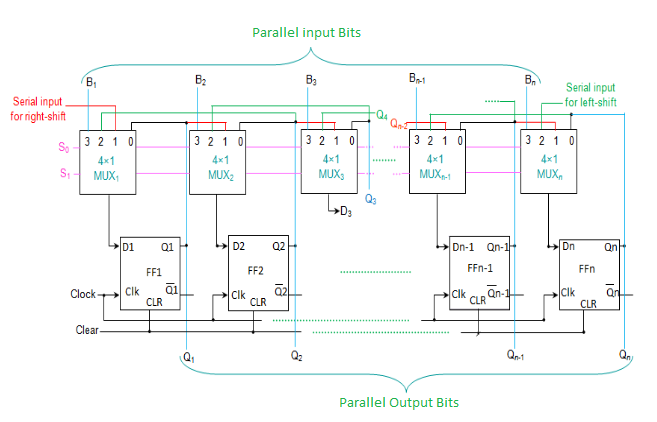
\includegraphics[width=0.8\textwidth]{imagens/universal shift register.png}
    \caption{Registrador de Deslocamento Universal (Fonte: Acervo Lima)}
    \label{fig:universal_sr}
\end{figure}

A palavra "UEFS", por sua vez, para ser representada em bits, foi utilizado a lógica presente na figura \ref{fig:uefs_em_bits}. Cada registrador terá em seu conjunto de flip-flops, na configuração da entrada paralela padrão, o bit representante da palavra "UEFS". Cada linha de bits da figura \ref{fig:uefs_em_bits} está representada como entrada do registrador. Por exemplo, o registrador da linha 1 (L1) possui, nas entradas de seus 16 flip-flops, a seguinte sequência de bits: 1010111011101110, respectivamente. 

\begin{figure}[!h]
    \centering
    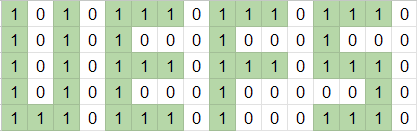
\includegraphics[width=0.5\textwidth]{imagens/palavra_em_bits.png}
    \caption{Representação em bits da palavra "UEFS"}
    \label{fig:uefs_em_bits}
\end{figure}

Cada flip-flop do tipo D recebe as seguintes entradas: ch0, ch1, para\_exibicao, dir\_esq, esq\_dir e CLK. Quando "para\_exibicao" for acionado (ch0 e ch1 em nível lógico baixo), os LEDs irão ser desligados e o registrador será setado com os valores iniciais pré-definidos. Quando "dir\_esq" for acionado (ch0 e ch1 em nível lógico alto e baixo, respectivamente), o flipflop atual vai receber a saída do flipflop anterior, ou seja, a exibição será feita da direita para a esquerda, pois será nessa orientação que os bits serão deslocados. Quando "esq\_dir" for acionado (ch0 e ch1 em nível lógico baixo e alto, respectivamente), o flipflop atual vai receber a saída do flipflop posterior, ou seja, a exibição será feita da esquerda para a direita, pois será nessa orientação que os bits serão deslocados. Por fim, quando ambas as entradas ch0 e ch1 forem nível lógico alto, o clock será inibido, ou seja, não haverá deslocamento e o painel será "pausado". O componente responsável por direcionar as entradas de seleção ch0 e ch1 para o flip-flop é o multiplexador. Por fim, os registradores enviam 7 saídas para a main, entituladas colunas, que são enviadas para a matriz de LEDs, que as selecionam através de um contador e um multiplexador.

Por sua vez, o módulo de matriz de LEDs é controlado por um contador e selecionador de linhas e colunas. O módulo recebe 2 sinais de entrada: ch0 e ch1, que são utilizados para habilitar ou desabilitar a matriz de LEDs. Há também um sinal de entrada CLK para sincronizar a operação do contador. Além disso, existem 35 sinais de entrada (C1L1, C1L2, ..., C7L5) que controlam os LEDs individuais e 12 sinais de saída (L1, L2, L3, L4, L5, C1, C2, C3, C4, C5, C6, C7) que são conectados aos pinos do componente físico.

O módulo utiliza um contador (Contador inst1) para selecionar a linha e a coluna correspondente que deve ser exibida na matriz de LEDs de maneira sicronizada. O contador gera três sinais de saída (en1, en2 e en3) que são usados para selecionar a linha e a coluna correspondente. A linha é selecionada com as portas lógicas AND que produzem um sinal alto (1) em cada linha correspondente selecionada, enquanto que as colunas são selecionadas por multiplexadores (MUXParaColuna) que conectam as saídas de cada coluna correspondente aos pinos de saída da matriz de LEDs.

O módulo também inclui uma função de habilitação/desabilitação, onde o sinal de saída "enable" é controlado pelos sinais de entrada ch0 e ch1. Se ambos forem zero, o "enable" é definido como zero, o que desabilita a matriz de LEDs. Caso contrário, o "enable" é definido como um sinal lógico alto (1), o que habilita a matriz de LEDs.

\begin{figure}
    \centering
    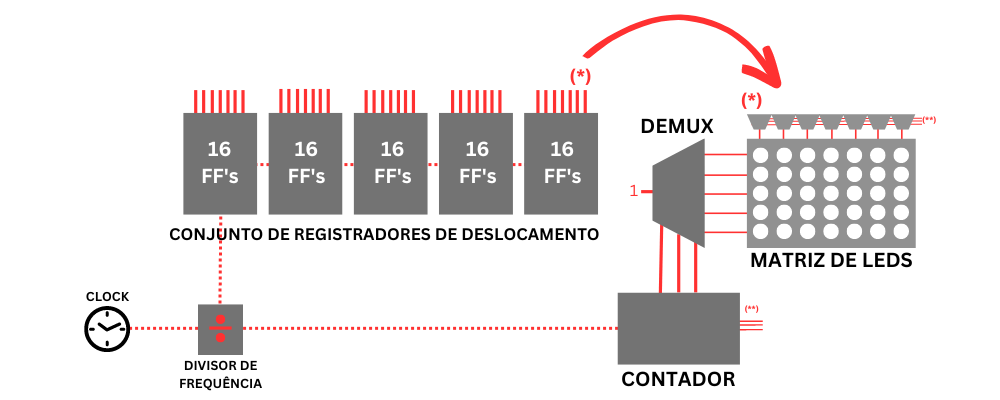
\includegraphics[width=0.9\textwidth]{imagens/design letreiro.png}
    \caption{Modelagem do circuito completo do painel eletrônico digital}
    \label{fig:modelagem}
\end{figure}

\section{Implementação física}

A implementação do código escrito em Verilog deve ser repassada para os circuitos integrados de lógica programável complexa (CPLD) para utilização do protótipo físico. 

Os CPLDs tem um funcionamento interno semelhante, mas mais complicados, aos integrados PAL e PLD. No CPLD existem vários sub-circuitos interconectados por uma matriz programável de interconexão global. Esses sub-circuitos recebem a nomenclatura de Logic Array Blocks (LABs) (Figura \ref{fig:diagramadeblocos}). Cada LAB contém blocos de I/O (entrada/saída), um circuito de expansão de termo produto e a quantidade de 4 a 16 macrocélulas. Cada macrocélula é estruturada com uma matriz AND conectada a uma matriz OR, para a implementação de soma de produtos, e flip-flops que, em alguns casos, são responsáveis pela realimentação de sinais na matriz AND \cite{CLPDarquitetura} O modelo utilizado foi o CPLD MAX II EPM240T100C5N.

Quando o código é ainda compilado no Quartus, uma série de informações acerca da implementação são geradas. No resumo do uso de recursos do Fitter, é possível ver todas essas informações. A partir do código apresentado neste relatório, temos as seguintes informações: 120/240 (50\%) elementos lógicos foram utilizados, todos no modo normal. Desses, no uso de elemento lógico por número de entradas LUT, 82 são de 4 entradas, 9 são de 3 entradas, 3 são de 2 entradas e 26 são de 1 entrada. Por fim, são utilizados 15 pinos, de 80 disponíveis (19\%).

\begin{figure}[!h]
  \centering
    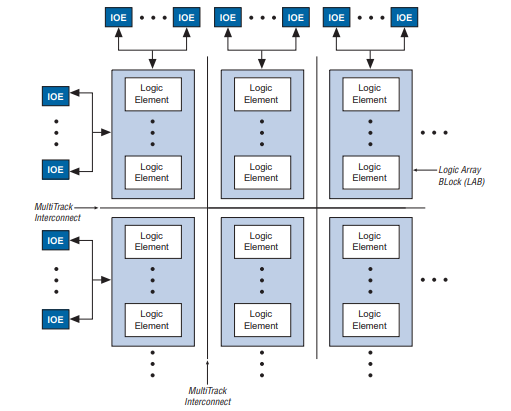
\includegraphics[width=0.45\textwidth]{imagens/diagrama.png}
  \caption{Diagrama de blocos do dispositivo MAX II}
  \label{fig:diagramadeblocos}
\end{figure}

\section{Teste e simulação}

Para realizar os testes físicos na placa, é recomendável realizar algumas simulações virtuais inicialmente e testar as saídas, na tentativa de perceber os problemas antes de estarem conectadas na placa. Caso a simulação esteja correta, o ideal é que a aplicação física tenha um resultado adequado. 

No momento de testes na placa, foi percebido uma anômalidade, onde os bits eram deslocados, mas não eram exibidos na matriz de maneira que desse para efetuar a leitura. Com uma análise, o problema foi visto na frequência que os bits eram exibidos. Em um divisor de frequência incial, os bits não eram exibidos adequadamente. Para verificar se o problema era realmente no divisor de frequência, uma saída foi forçada para o relé do kit de desenvolvimento LEDS CPLD, que foi conectada ao osciloscópio. Com isso, foi analisado que o clock do sistema não estava sendo dividido. Um erro foi diagnosticado no código e corrigido. Após isso, os testes foram validados e executados de maneira esperada, como demonstrada a seguir:

\begin{equation} \label{eqCLK2}
    x=\frac{50000000}{2^5}
\end{equation}

\begin{figure}[!h]
    \centering
    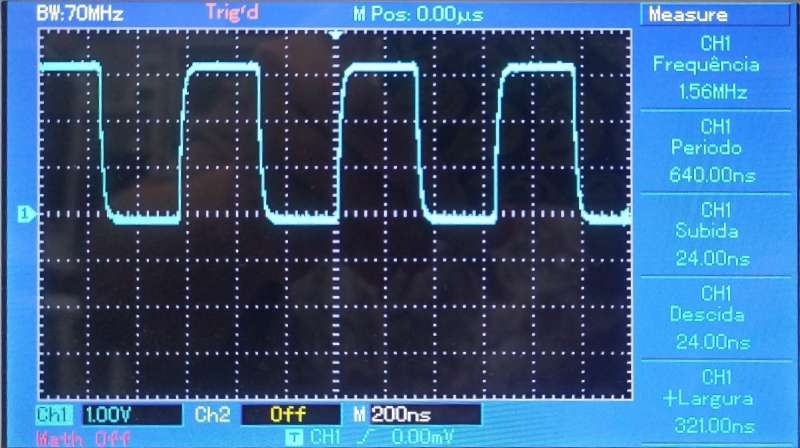
\includegraphics[width=0.6\textwidth]{imagens/osci01.jpg}
    \caption{Teste da divisão de frequência em 5 Flip-Flops feito no osciloscópio.}
    \label{fig:osci5}
\end{figure}

Dividindo o clock em 5 Flip-Flops, como demonstrado na equação \ref{eqCLK2}, para a sua utilização na matriz de LEDs, o resultado chega a 1562500Hz, ou 1,56MHz. A figura \ref{fig:osci5} demonstra o teste feito utilizando o osciloscópio. Para a realização do teste, foram utilizadas as saídas do relé do kit de desenvolvimento (LEDS CPLD). Essas saídas foram conectadas ao osciloscópio para demonstração da divisão do clock.

\begin{equation} \label{eqCLK3}
    x=\frac{50000000}{2^2^3}
\end{equation}

\begin{figure}
    \centering
    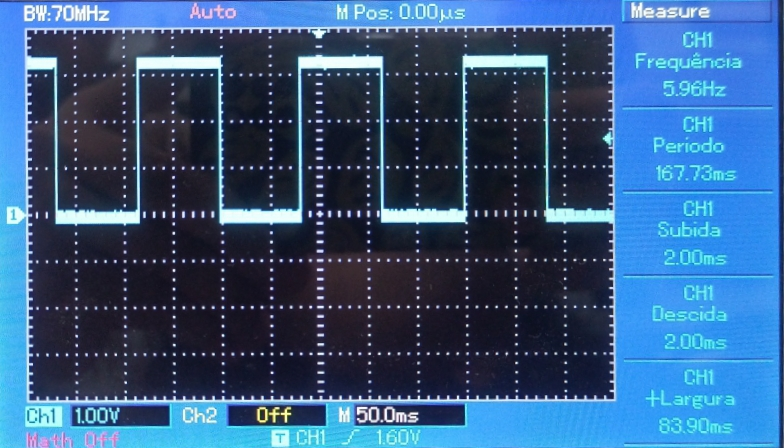
\includegraphics[width=0.6\textwidth]{imagens/osci02.jpg}
    \caption{Teste da divisão de frequência em 23 Flip-Flops feito no osciloscópio.}
    \label{fig:osci23}
\end{figure}

Já o clock que foi utilizado para o registrador de deslocamento, precisou ser utilizar 23 Flip-Flops no divisor de frequência, como demonstrado na equação \ref{eqCLK3}, com o resultado chegando a aproximadamente 5,96Hz. O resultado precisa ser menor que o clock de exibição da matriz pois o deslocamento precisa ser percptível referente a sua exibição. A figura 6 demonstra o teste feito utilizando o osciloscópio.


